\documentclass[11pt]{article}
\usepackage[a4paper,margin=2.5cm]{geometry}
\usepackage[english]{babel}
\usepackage{amsmath}
\usepackage{graphicx}

\title{Heuristic analysis for the knights-isolation game}
\author{Abderrahim Kitouni}

\begin{document}
\maketitle

I propose three evaluation functions in addition to the one proposed in the assignment, which is defined by
\[
  improved\_score =
  \begin{cases}
    +\infty, & \text{ if player won} \\
    -\infty, & \text{ if player lost} \\
    \#player\_moves - \#opponent's\_moves, & \text{ otherwise}
  \end{cases}
\]

My proposals for evaluation functions are incremental improvements over this. First, $custom\_score\_3$ is defined as follows
\[
  custom\_score\_3 =
  \begin{cases}
    +\infty, & \text{ if player won} \\
    -\infty, & \text{ if player lost} \\
    2 \times \#player\_moves - \#opponent's\_moves, & \text{ otherwise}
  \end{cases}
\]
This puts more emphasis on the number of moves available for the player and less on reducing the number of moves the opponent can make. This should produce less aggressive play than $improved\_score$, but I noticed slightly better results.

The second, $custom\_score\_2$, is defined as follows
\[
  custom\_score\_2 =
  \begin{cases}
    +\infty, & \text{ if player won} \\
    - 2 \times board\_size + turn\_number, & \text{ if player lost} \\
    2 \times \#player\_moves - \#opponent's\_moves, & \text{ otherwise}
  \end{cases}
\]
The difference with $custom\_score\_3$ is that it gives different scores for different losing positions. When the agent determines that it's going to lose if the other player plays optimally, instead of forfeiting (or selecting a random move), it tries to make the game last as much as possible in the hope that the other player makes a mistake. This works well against weaker agents, but not so much against agents that use alpha-beta pruning as these will have searched to end-game at that point.

The last proposal, $custom\_score$ is defined by
\[
  custom\_score =
  \begin{cases}
    +\infty, & \text{ if player won} \\
    - 2 \times board\_size + turn\_number, & \text{ if player lost} \\
    \#player\_moves - \frac{1}{2} \log(turn\_number) \times \#opponent's\_moves, & \text{ otherwise}
  \end{cases}
\]
The reasoning behind this is that the agent will simply look for open space at the beginning of the game, and starts being more aggressive as the game progresses. This seemed a good idea at first, and showed promising results on small number of trials. Running it on a larger number of trials showed that the difference isn't significant.

Here the results obtained from running a tournament. The same agent using iterative deepening with alpha-beta pruning and each of the above heuristics is run against seven opponents. Each pair played 100 ``fair'' matches. That is, from a random starting positions each agent plays as first player then as second player. To make sure there isn't much variance, the tournament was run three times, resulting in 600 playouts in total.

In order not to clutter the chart, I divided the opponents into three categories: weak opponents, which are the random player and the limited-depth minimax player with the distance-from-centre heuristic; medium opponents which are the limited-depth minimax players with better heuristics; and finally AB opponents which use iterative-deepening with alpha-beta pruning.

\begin{figure}\label{chart}
  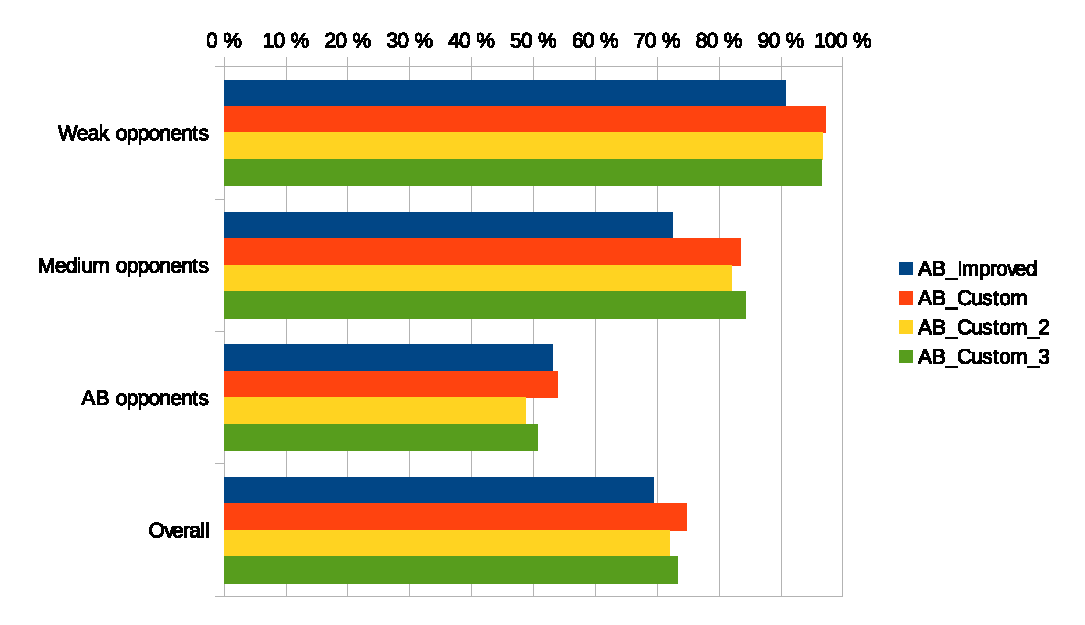
\includegraphics[width=\textwidth]{chart.eps}
\end{figure}

The chart shows that there isn't much difference between the different heuristics when playing against agents that search deep in the game tree. However, there is a clear advantage against weaker agents for using a heuristic score that depends on the length of the game.
\end{document}
